\section{Problem Introduction}

The project, which is aimed at investigating the potential of 3D metallic printing using WAAM, is focused on an Iron-Cobalt (Fe-Co) alloy called Vacoflux-17 known for its superior magnetic properties.

Vacoflux 17 is a type of Fe-Co alloy that has excellent magnetic properties and can be used for high performance magnetic actuators. It is produced by VACUUMSCHMELZE GmbH \& Co. KG, a company that specializes in advanced magnetic solutions.
Vacoflux 17 can be supplied in various forms, such as strip material, stamped parts, solid rods, and wire material. It has a saturation polarization of 2.22 T, an electrical resistivity of 0.41 $\mu \Omega m$, and a Curie temperature of 920 °C.

It can be heat treated in hydrogen atmosphere to improve its mechanical properties and reduce its iron losses. Vacoflux 17 is suitable for applications such as components and actuators for the automotive industry, especially diesel injection, and rotors and stators of electrical motors and generators.

The overarching goal of the investigation is to manufacture simple multilayer geometries that retain the material's base mechanical and magnetic properties with a minimum finish quality and geometric accuracy.

Inititally in the internship, the processability of the Fe-Co alloy is to be evaluated and its microstructural evolution during deposition using WAAM is to be understood. This involves conducting a series of experiments to observe the alloy's behavior under various conditions and analyzing the resulting depositions. The objective is to acquire a comprehensive understanding of how the alloy reacts to the WAAM process and how its properties are altered by deposition.

The focus then transitions towards developing deposition procedures that enable successful 3D printing of the Fe-Co alloy. This involves further experimentation and analysis, with an emphasis on optimizing process parameters to achieve desired material properties. The final part of this stage involves characterizing the material properties of the printed Fe-Co alloy, including its magnetic properties.

Throughout both stages, supervision is provided by experts from RAMLAB and TU Delft. Training in relevant techniques and methodologies is received, a thorough literature review is conducted, experiments are carried out, and results are analyzed. This project offered a unique opportunity to gain hands-on experience in 3D metallic printing and contribute to cutting-edge research in this field.

\section{Literature Review and Background Information}

\subsection{MIG WAAM}

(Metal Inert Gas) MIG WAAM consists depositing molten wire onto a workpiece using an electric arc between the wire and workpiece as a heat source. MIG welding uses inert gases for shielding and is suitable for non-ferrous metals like aluminum, while MAG (Metal Active Gas) welding uses active gas mixtures and is used for welding steel.

MIG and MAG differ from the other two main welding methods: TIG (Tungsten Inert Gas) welding uses an open arc shielded by inert gases like argon or helium, while PAW (Plasma Arc Welding) uses a constricted arc with the electrode positioned within the torch body, separating the plasma arc from the shielding gas envelope.

The main phases of MIG deposition are as follows:

\begin{enumerate}
    \item Arc Generation: The process begins with the generation of an electric arc between the wire electrode and the workpiece. This arc is hot enough to melt the wire electrode and part of the workpiece.
    \item Melting and Deposition: The melted wire, now in a liquid state, is then deposited onto the workpiece in a selective layered fashion.
    \item Solidification: Upon the solidification of the molten metal layer over a cold substrate, the subsequent thermal contraction of the metal layer generates tensile and compressive stresses respectively on the deposited layer and substrate.
    \item Heat Transfer and Fluid Flow: The heat transfer and fluid flow during this process play a crucial role in determining the final microstructure and mechanical properties of the deposited material.
\end{enumerate}

\subsubsection{Process parameters}

The main process parameters in MIG are current/wire feed rate, voltage, and travel speed, and wire feed rate, affect the bead geometry, mechanical properties, and deposition rate of the produced parts.


\textbf{Voltage} in welding primarily affects the width of the weld bead and the amount of spatter. Higher voltage settings result in a wider weld bead and more spatter.

The \textbf{welding current} affects the heat available to melt the welding wire and the base material. It is directly correlated to wire \textbf{feed rate}: when feed rate increases, so does the welding amperage. Higher amperage settings yield greater joint penetration.

\textbf{Travel speed} in welding primarily affects the size of the weld bead and heat input. An increase in travel speed leads to a decrease in heat input, resulting in a narrower weld bead and a smaller heat-affected zone. However, increasing the travel speed beyond a certain limit can lead to insufficient fusion and porosity in the weld. Conversely, slow travel speeds can cause excessive weld deposition, which commonly causes cold lapping or a lack of fusion.



\subsubsection{Cold Metal Transfer (CMT)}

CMT, or Cold Metal Transfer, is a welding process developed by Fronius that stands out due to its extremely low heat input and an significantly stable arc. The method boasts less distortion, 50\% less dilution of filler and base material, and higher welding speeds.
The digital process control detects a short circuit (wire touching workpiece) and then detaches the droplet by retracting the wire. During welding, the wire moves forward and is pulled back again as soon as the short circuit occurs, as shown in \autoref{fig:CMT}. Several different waveforms for this process have been developed, often catering to the different needs of specific materials, like NiCr, steel, and Al.
As a result, the arc only introduces any heat for a very brief period during the arc-burning phase. The short circuit is controlled and the current is kept low, resulting in a nearly spatter-free material transfer. The arc length is detected and adjusted mechanically. The arc remains stable, no matter what the surface of the workpiece is like or how fast the user welds.

\begin{minipage}{\linewidth}
    \centering
    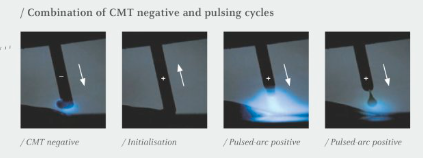
\includegraphics[width=\linewidth]{images/CMT_illustration.PNG}
    \captionof{figure}{CMT cycle}
    \label{fig:CMT}
\end{minipage}


\subsection{Soft Magnetic Materials}

Soft magnetic materials are materials that are easy to be magnetized and demagnetized, whereas hard magnetic materials keep their magnetization and are often permanent magnets.

\subsubsection{Magnetic property definitions}

\textbf{Saturation magnetization} occurs when an increase in the applied magnetic field no longer increases the magnetization of a material. This is due to the alignment of magnetic domains reaching their maximum, resulting in a leveling off of the total magnetic flux density.

\textbf{Magnetic coercivity}, also known as coercive force, is a measure of a ferromagnetic material's ability to resist demagnetization from an external magnetic field. It is measured in oersted or ampere/meter units. There are different types of coercivity, including normal coercivity, intrinsic coercivity, and remanence coercivity, each representing different aspects of demagnetization.

\textbf{Magnetic permeability}, denoted by the Greek letter \(\mu\), measures how a material reacts to a magnetic field. It is the ratio of the magnetic flux density established within the material to the magnetic field strength of the magnetizing field. In simpler terms, it indicates a material's ability to support the development of a magnetic field and its resistance to that field.

\textbf{Magnetic power losses}, also known as iron losses, occur in the core of magnetic components like transformers and inductors. These losses are caused by hysteresis and eddy currents. Hysteresis loss happens when a magnetic material lags behind changes in the magnetic field, dissipating energy as heat. Eddy current loss occurs due to induced currents in the core, producing heat. These losses impact the efficiency of electromagnetic devices, making their reduction crucial in device design.

The \textbf{Curie temperature} is the temperature at which materials lose their permanent magnetic properties and can be replaced by induced magnetism. At the Curie temperature, a material's intrinsic magnetic moments change direction, causing a transition from ordered to disordered magnetic moments.

\subsubsection{Properties of SMMs}

Soft magnetic materials possess several desirable properties that make them suitable for various applications.

High saturation magnetization: being able to store a significant amount of magnetic energy, makes them efficient for applications such as transformers, inductors, and magnetic storage devices. This property allows them to generate strong magnetic fields when exposed to an external magnetic field.

Low coercivity: they can easily switch their magnetization direction when subjected to an external magnetic field. This property is crucial for applications that require rapid magnetization and demagnetization cycles, such as in transformers and electric motors. Low coercivity ensures efficient energy conversion and reduces energy losses.

High initial/maximum permeability ($\mu_{max}$): they can quickly respond to changes in the magnetic field, allowing for efficient magnetic flux induction. This property is essential for applications like electromagnetic shielding, where the material needs to redirect magnetic fields away from sensitive components.

Low power losses.

High Curie temperature: they can magnetic properties at elevated temperatures. This property is desirable for applications that involve high-temperature environments, such as power electronics, where the material needs to retain its magnetic characteristics even under thermal stress.

\subsubsection{Fe-Co alloys}

Fe-Co alloys, depending on the manufacturing method, can be either amorphous or nanocrystalline. Amorphous and nanocrystalline soft magnetic materials have superior magnetic properties and durability compared to normal soft magnetic alloys. They exhibit lower coercivity, higher permeability, and lower eddy current losses, making them more efficient for power electronics and electrical machines.

Fe-Co alloys can have both the alpha and gamma phases, with the alpha phase being a solid solution based on the body-centered cubic structure and the alpha' phase being an ordered intermetallic phase formed by the primary crystallization of the amorphous alloy. The alpha' phase contributes to the excellent soft magnetic properties of the alloy.

\subsubsection{Microstructure and magnetic properties}

The microstructure of a material has a significant impact on its magnetic properties. Several key factors should be taken into account:

\textbf{Grain structure}: The arrangement of grains in the material can greatly influence its magnetic behavior. Different types of grain structures, such as planar, cellular, columnar dendritic, and equiaxed dendritic, can result in varying magnetic properties.

\textbf{Grain size}: The size of the grains also plays a role. For example, in FePt storage films used in heat-assisted magnetic recording media, the grains need to be smaller than 6 nm to achieve a specific areal density.

\textbf{Phase composition}: The composition of different phases within the material can affect its magnetic properties. In some cases, a microstructure with uniformly dispersed nanocrystals of specific compositions has been found to optimize magnetic properties.

% \textbf{Processing conditions}: The conditions under which the material is processed can impact its microstructure and, consequently, its magnetic properties.

\textbf{Microstructural features}: Certain features within the microstructure can enhance or diminish magnetic properties. For instance, complex microstructures tend to have higher coercivity and lower remanence than simple ones.

\subsection{Characterization techniques}

\subsubsection{Weld Characterization}



\subsubsection{Magnetic Characterization}

\subsection{Post treatment techniques}

\subsection{Previous work}



